\subsection{UC5 - Gestione delle cartelle di cui viene effettuato il backup}
\begin{figure}[H]
    \centering
    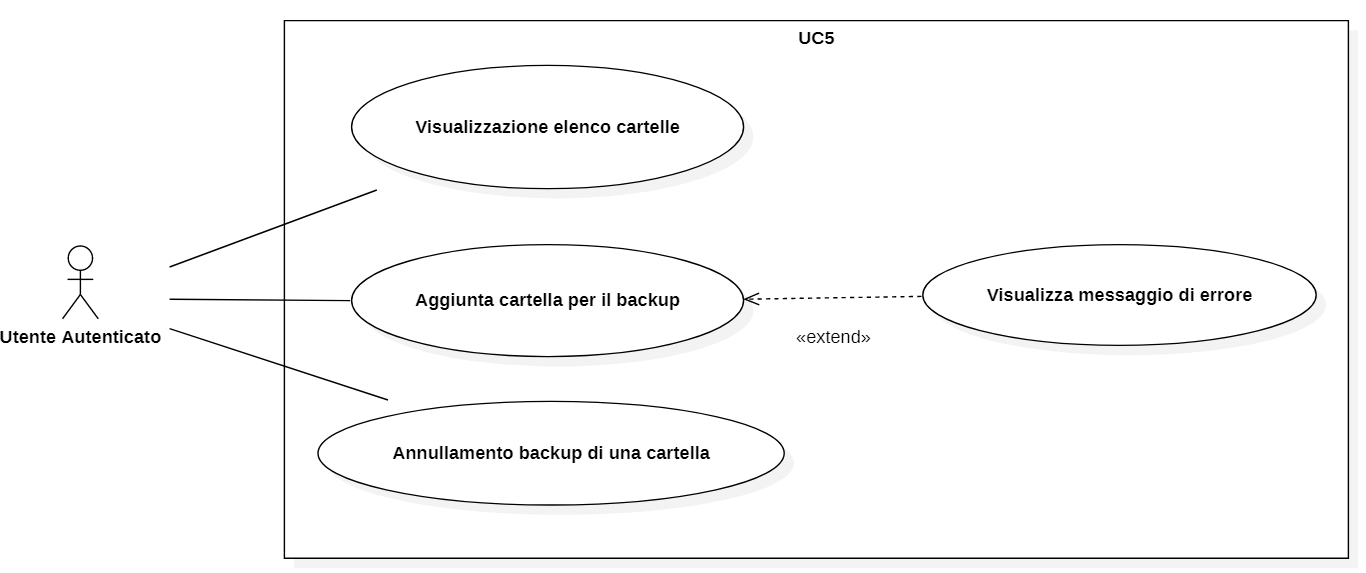
\includegraphics[scale = 0.4]{components/img/UC5.png}
    \caption{UC1 - Autenticazione}
\end{figure}
\begin{itemize}
\item \textbf{Attore Primario:} Utente autenticato;
\item \textbf{Precondizione:} L'utente ha a disposizione varie funzionalità per la gestione delle cartelle di cui viene effettuato il backup;
\item \textbf{Postcondizione:} Viene eseguita l'operazione selezionata dall'utente;
\item \textbf{Scenario principale:}
    \begin{enumerate}
    \item L'utente può visualizzare l'elenco delle cartelle di cui viene effettuato il backup;
    \item L'utente può aggiungere una nuova cartella per il backup;
    \item L'utente può annullare il backup di una cartella.
    \end{enumerate}
\item \textbf{Estensioni:}
\begin{itemize}
\item L'utente cerca di aggiungere una cartella non idonea (ad esempio, cartelle di sistema o cartelle presenti su un dispositivo di rete);
\item L'utete cerca di aggiungere una cartella che ha lo stesso identificativo di una già sincronizzata.
\end{itemize}
\end{itemize}